\subsection{Galileo’s Big Shot: From Cannonballs to Inertia}

\textbf{Aristotle (4th century BCE)} had taught that \textbf{heavier objects fall faster} than lighter ones because they have a greater “natural motion.” This belief went unchallenged for centuries until \textbf{Galileo Galilei (1600s)} decided to put it to the test.

Galileo was fascinated by cannonballs and their curved trajectories. Cannons, a new and powerful weapon in Renaissance warfare, provided a perfect testing ground for the physics of motion.

He made a key observation:

\begin{itemize}
    \item Cannonballs don’t travel in a straight line when fired. Instead, they \textbf{arc downward over time}.
    \item The longer they travel, the \textbf{steeper their descent} becomes.
    \item The path of a cannonball is a \textbf{parabola}—a shape he could describe mathematically.
\end{itemize}

\begin{center}
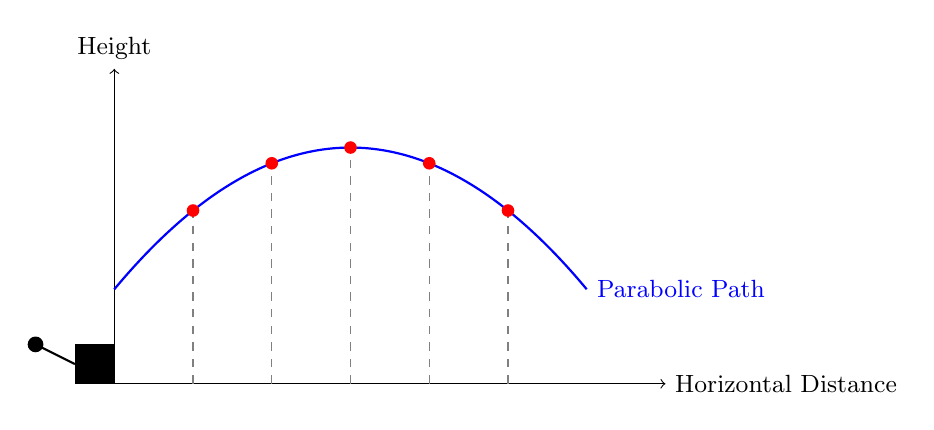
\begin{tikzpicture}
    % Axes
    \draw[->] (0,0) -- (7,0) node[right] {\small Horizontal Distance};
    \draw[->] (0,0) -- (0,4) node[above] {\small Height};

    % Cannon
    \fill[black] (-0.5,0) rectangle (0,0.5);
    \draw[thick] (-0.5,0.25) -- (-1,0.5); % Cannon barrel
    \fill[black] (-1,0.5) circle (0.1); % Cannonball before firing

    % Parabolic Trajectory
    \draw[thick, blue, domain=0:6, samples=50, smooth, variable=\x] plot ({\x},{-0.2*(\x-3)*(\x-3)+3}) node[right] {\small Parabolic Path};

    % Dotted Lines for motion steps
    \foreach \x in {1,2,3,4,5} {
        \draw[dashed, gray] (\x,0) -- (\x,{-0.2*(\x-3)*(\x-3)+3});
        \fill[red] (\x,{-0.2*(\x-3)*(\x-3)+3}) circle (0.08); % Cannonball positions
    }

\end{tikzpicture}
\end{center}


Which was all well and good. But here’s the thing: this wasn’t just an interesting observation about flying death spheres. It was also a direct contradiction of \textbf{Aristotle}, who had been the gold standard for physics (and, by this time, Catholic doctrine) for centuries. 

See, Aristotle thought motion worked like this:
\begin{itemize}
    \item Things move because something \textbf{pushes} them.
    \item Once that push stops, they slow down and come to a halt.
    \item If they go up, they must eventually come down because, you know, \textbf{nature just works that way}.
\end{itemize}

Galileo, however, had the audacity to suggest that objects don’t just stop on their own: \textbf{they keep moving unless something stops them}. And when it came to projectiles? He discovered something even more radical.

To investigate further, he constructed ramps and rolled balls down them at different angles. He found that:

\begin{itemize}
    \item \textbf{Objects in free fall accelerate}: The longer they fall, the faster they go.
    \item The \textbf{horizontal and vertical motions of a projectile are independent}:
    \begin{itemize}
        \item A cannonball fired forward moves \textbf{horizontally at a constant speed}.
        \item Meanwhile, it \textbf{accelerates downward under gravity}.
    \end{itemize}
\end{itemize}

These two motions combine to create a \textbf{curved trajectory}. Which meant that Aristotle was wrong. And Galileo, being Galileo, wasn’t exactly subtle about pointing it out.

\begin{figure}[H]
\centering
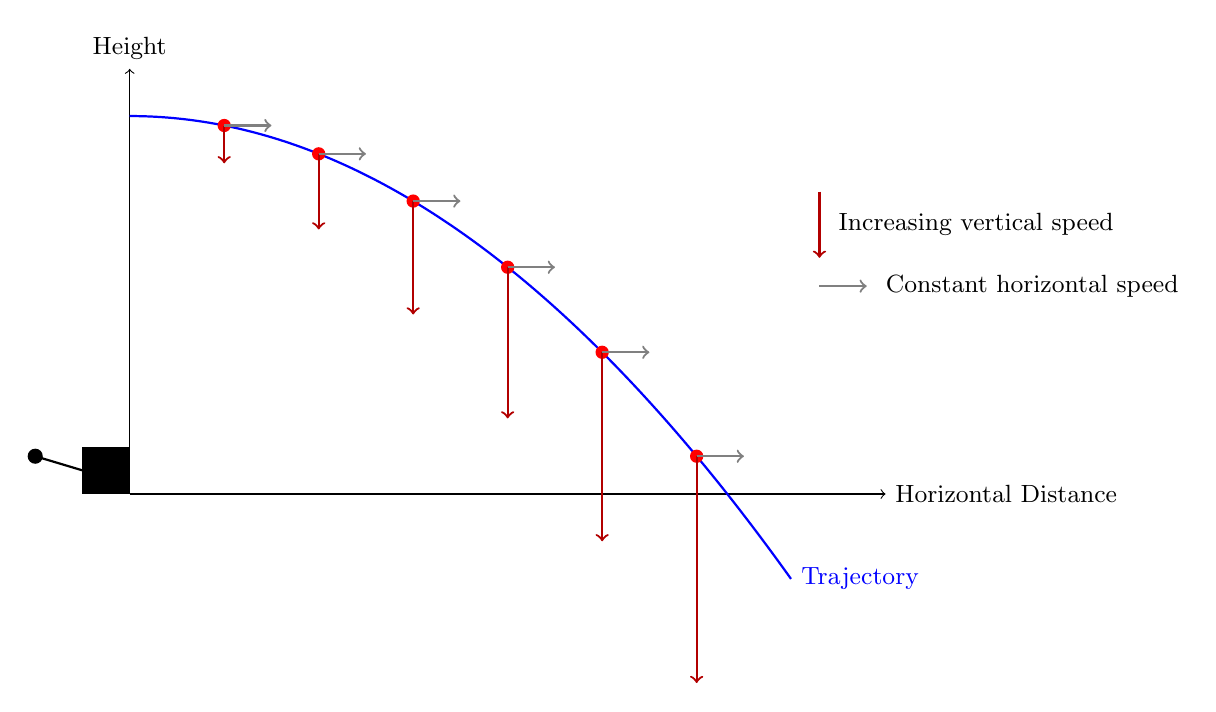
\begin{tikzpicture}[scale=1.2]
    % Axes
    \draw[->] (0,0) -- (8,0) node[right] {\small Horizontal Distance};
    \draw[->] (0,0) -- (0,4.5) node[above] {\small Height};

    % Cannon (simple rectangle and barrel)
    \fill[black] (-0.5,0) rectangle (0,0.5);
    \draw[thick] (-0.5,0.25) -- (-1,0.4);
    \fill[black] (-1,0.4) circle (0.08); % Cannonball before firing

    % Parabolic trajectory
    \draw[thick, blue, domain=0:7, smooth, samples=100, variable=\x] 
        plot ({\x}, {4 - 0.1*\x*\x}) node[right] {\small Trajectory};

    % Time steps with red cannonballs and vertical velocity arrows
    \foreach \t in {1,2,3,4,5,6} {
        \pgfmathsetmacro{\y}{4 - 0.1*(\t*\t)}
        \fill[red] (\t, \y) circle (2pt);
        \draw[->, thick, red!70!black] (\t, \y) -- (\t, {\y - 0.4*\t});
    }

    % Horizontal velocity arrows (gray)
    \foreach \t in {1,2,3,4,5,6} {
        \pgfmathsetmacro{\y}{4 - 0.1*(\t*\t)}
        \draw[->, thick, gray] (\t, \y) -- ({\t + 0.5}, \y);
    }

    % Legend
    \draw[->, thick, red!70!black] (7.3,3.2) -- (7.3,2.5);
    \node[right] at (7.4,2.85) {\small Increasing vertical speed};

    \draw[->, thick, gray] (7.3,2.2) -- (7.8,2.2);
    \node[right] at (7.9,2.2) {\small Constant horizontal speed};

\end{tikzpicture}

\vspace{0.5em}
\caption{\small Galileo understood projectile motion as the combination of two independent effects: constant horizontal motion and accelerated vertical fall. From his ramp experiments, he observed that falling bodies accelerate over time. When a cannonball is fired horizontally, it continues moving forward at a steady rate while simultaneously accelerating downward due to gravity. These two motions combine to produce a curved, parabolic trajectory — a clear contradiction to Aristotle’s claim that all motion requires a continuous cause.}
\end{figure}


\textbf{But this discovery had an even bigger consequence} because Galileo wasn’t just playing with cannonballs; he was laying the foundation for why the Earth could move around the Sun without us noticing. The standard objection to heliocentrism was simple: 

\begin{quote}
    \textbf{If the Earth is moving, why don’t we feel it?}
\end{quote}

Aristotle’s physics made it clear: motion required a cause, and objects naturally came to rest. If Earth were truly spinning at high speeds and hurtling around the Sun, wouldn’t everything be flying off the surface? 

\textbf{But Galileo’s ramp experiments held the answer: inertia.}

\begin{itemize}
    \item Once an object is in motion, it \textbf{stays in motion} unless acted upon by an external force.
    \item That meant that if Earth were moving, \textbf{everything on it would be moving too}.
    \item Just as a ball rolling on a smooth surface keeps going without slowing down, people, air, and objects on Earth would all \textbf{share its motion}.
\end{itemize}

\begin{figure}[H]
\centering
\begin{tikzpicture}[every node/.style={font=\footnotesize}]

% Panel 1 — Galileo explains inertia
\comicpanel{0}{4}
  {Galileo}
  {Aristotle}
  {\textbf{Galileo:} I rolled a ball down a ramp. The flatter the surface, the longer it moved. I think motion continues unless something stops it.}
  {(0,-0.5)}

% Panel 2 — Aristotle looks unimpressed
\comicpanel{6.5}{4}
  {Aristotle}
  {Galileo}
  {\textbf{Aristotle:} So... you’re saying a rock just keeps moving? On its own? That’s absurd. Motion needs a purpose.}
  {(0,-0.5)}

% Panel 3 — Galileo is confused
\comicpanel{0}{0}
  {Galileo}
  {Aristotle}
  {\textbf{Galileo:} It doesn't need a purpose. It just keeps going. That’s inertia.}
  {(0,0.8)}

% Panel 4 — Aristotle lands the punchline
\comicpanel{6.5}{0}
  {Aristotle}
  {Student}
  {\textbf{Aristotle:} Motion without purpose? Might as well say the rock has free will.}
  {(0,0.8)}

\end{tikzpicture}
\caption{Inertia: the radical idea that objects don’t need permission to keep moving.}
\end{figure}


